\documentclass[a4paper, 12pt]{article}		% general format
\usepackage{multicol}
%%%% Charset
\usepackage{cmap}							% make PDF files searchable and copyable
\usepackage[utf8x]{inputenc} 				% accept different input encodings
\usepackage[english,russian]{babel}   %% загружает пакет многоязыковой вёрстки
\usepackage{fontspec}      %% подготавливает загрузку шрифтов Open Type, True Type и др.
\defaultfontfeatures{Ligatures={TeX},Renderer=Basic}  %% свойства шрифтов по умолчанию
\setmainfont[Ligatures={TeX,Historic}]{Roboto-Light} %% задаёт основной шрифт документа
\setsansfont{Roboto-Light}  
\usepackage{float}
%%%% Graphics
\usepackage[dvipsnames]{xcolor}			% driver-independent color extensions
\usepackage{graphicx}						% enhanced support for graphics
\usepackage{wrapfig}						% produces figures which text can flow around

%%%% Math
\usepackage{amsmath}						% American Mathematical Society (AMS) math facilities
\usepackage{amsfonts}						% fonts from the AMS
\usepackage{amssymb}						% additional math symbols

%%%% Typograpy (don't forget about cm-super)
\usepackage{microtype}						% subliminal refinements towards typographical perfection
\linespread{1.3}							% line spacing
\usepackage[left=2.5cm, right=1.5cm, top=2.5cm, bottom=2.5cm]{geometry}
\setlength{\parindent}{0pt}					% we don't want any paragraph indentation
\usepackage{parskip}						% some distance between paragraphs

%%%% Tables
\usepackage{tabularx}						% tables with variable width columns
\usepackage{multirow}						% for tabularx
\usepackage{hhline}							% for tabularx
\usepackage{tabu}
\usepackage{longtable}

%%%% Graph
\usepackage{tikz}							% package for creating graphics programmatically
\usetikzlibrary{arrows}						% edges for tikz

%%%% Other
\usepackage{url}							% verbatim with URL-sensitive line breaks
\usepackage{fancyvrb}						% sophisticated verbatim text (with box)

\usepackage{listings}
\usepackage{caption}
\DeclareCaptionFont{white}{\color{white}}
\DeclareCaptionFormat{listing}{\colorbox{gray}{\parbox{\dimexpr\textwidth-1.72\fboxsep\relax}{#1#2#3}}}
\captionsetup[lstlisting]{format=listing,labelfont=white,textfont=white,margin=0pt}
\lstset{language=C,
	basicstyle=\footnotesize,
	keepspaces=true,
	tabsize=4,               
	frame=single,                           % Single frame around code
	rulecolor=\color{black},
	captionpos=b,
	showstringspaces=false,	
	abovecaptionskip=-0.9pt,
	xleftmargin=3.4pt,
	xrightmargin=2.6pt,
	breaklines=true,
	postbreak=\raisebox{0ex}[0ex][0ex]{\ensuremath{\color{black}\hookrightarrow\space}},
	xleftmargin=3.2pt,
	literate={а}{{\selectfont\char224}}1
	{~}{{\textasciitilde}}1
	{б}{{\selectfont\char225}}1
	{в}{{\selectfont\char226}}1
	{г}{{\selectfont\char227}}1
	{д}{{\selectfont\char228}}1
	{е}{{\selectfont\char229}}1
	{ё}{{\"e}}1
	{ж}{{\selectfont\char230}}1
	{з}{{\selectfont\char231}}1
	{и}{{\selectfont\char232}}1
	{й}{{\selectfont\char233}}1
	{к}{{\selectfont\char234}}1
	{л}{{\selectfont\char235}}1
	{м}{{\selectfont\char236}}1
	{н}{{\selectfont\char237}}1
	{о}{{\selectfont\char238}}1
	{п}{{\selectfont\char239}}1
	{р}{{\selectfont\char240}}1
	{с}{{\selectfont\char241}}1
	{т}{{\selectfont\char242}}1
	{у}{{\selectfont\char243}}1
	{ф}{{\selectfont\char244}}1
	{х}{{\selectfont\char245}}1
	{ц}{{\selectfont\char246}}1
	{ч}{{\selectfont\char247}}1
	{ш}{{\selectfont\char248}}1
	{щ}{{\selectfont\char249}}1
	{ъ}{{\selectfont\char250}}1
	{ы}{{\selectfont\char251}}1
	{ь}{{\selectfont\char252}}1
	{э}{{\selectfont\char253}}1
	{ю}{{\selectfont\char254}}1
	{я}{{\selectfont\char255}}1
	{А}{{\selectfont\char192}}1
	{Б}{{\selectfont\char193}}1
	{В}{{\selectfont\char194}}1
	{Г}{{\selectfont\char195}}1
	{Д}{{\selectfont\char196}}1
	{Е}{{\selectfont\char197}}1
	{Ё}{{\"E}}1
	{Ж}{{\selectfont\char198}}1
	{З}{{\selectfont\char199}}1
	{И}{{\selectfont\char200}}1
	{Й}{{\selectfont\char201}}1
	{К}{{\selectfont\char202}}1
	{Л}{{\selectfont\char203}}1
	{М}{{\selectfont\char204}}1
	{Н}{{\selectfont\char205}}1
	{О}{{\selectfont\char206}}1
	{П}{{\selectfont\char207}}1
	{Р}{{\selectfont\char208}}1
	{С}{{\selectfont\char209}}1
	{Т}{{\selectfont\char210}}1
	{У}{{\selectfont\char211}}1
	{Ф}{{\selectfont\char212}}1
	{Х}{{\selectfont\char213}}1
	{Ц}{{\selectfont\char214}}1
	{Ч}{{\selectfont\char215}}1
	{Ш}{{\selectfont\char216}}1
	{Щ}{{\selectfont\char217}}1
	{Ъ}{{\selectfont\char218}}1
	{Ы}{{\selectfont\char219}}1
	{Ь}{{\selectfont\char220}}1
	{Э}{{\selectfont\char221}}1
	{Ю}{{\selectfont\char222}}1
	{Я}{{\selectfont\char223}}1,
	extendedchars=true
}

%галочка
\usepackage{amssymb}% http://ctan.org/pkg/amssymb
\usepackage{pifont}% http://ctan.org/pkg/pifont
\newcommand{\cmark}{\ding{52}}%
\newcommand{\xmark}{\ding{56}}
%------------------------------------------------------------------------------
\renewcommand{\labelenumii}{\theenumii}
\renewcommand{\theenumii}{\theenumi.\arabic{enumii}.}
\begin{document}
%------------------------------------------------
	\begin{titlepage}
		\begin{center}
			\large {Санкт-Петербургский политехнический университет Петра Великого\\
				Институт компьютерных наук и технологий}\\
		\end{center}
		\begin{center}
			\large\textbf {Кафедра компьютерных систем и программных технологий}
		\end{center}
		\vfill
		\begin{center}
			\large{\textbf{Отчет о лабораторной работе №5} \\
			\textbf{Курс: } Администрирование компьютерных сетей\\
			\textbf{Тема: } Перенос сети в Cisco Packet Tracer}
		\end{center}
		
		\vfill
		
		\flushleft{Выполнил студент группы 13541/3} 
		\hfill\parbox{9 cm}{\hspace*{3cm}\hbox to 0cm{\raisebox{-1em}{\small(подпись)}}\hspace*{-0.8cm}\rule{3cm}{0.8pt} Д.В. Круминьш}\\[0.6cm]
		
		\flushleft{Преподаватель} \hfill\parbox{9 cm}{\hspace*{3cm}\hbox to 0cm{\raisebox{-1em}{\small(подпись)}}\hspace*{-0.8cm}\rule{3cm}{0.8pt} И.А. Малышев}\\[0.6cm]
		
		\vspace{\fill}
		\begin{center}
			Санкт-Петербург \\ 2018 г.
		\end{center}
	\end{titlepage}
%------------------------------------------------
\setcounter{page}{2}
%\tableofcontents
%\clearpage

%------------------------------------------------------------------------------
%\input{intro}
\section{Цели работы}
\begin{enumerate}
\item Ознакомиться с Cisco Packet Tracer, и выполнить в нем:
\begin{itemize}
\item Построение компьютерной сети(из прошлых работ);
\item Настроить сервисы DNS, DHCP, TFTP;
\item Выполнить тестирование сети.
\end{itemize}
\end{enumerate}

\section{Построение компьютерной сети}
Средствами Cisco Packet Tracer была построена следующая схема:
\begin{figure}[H]
  \centering
  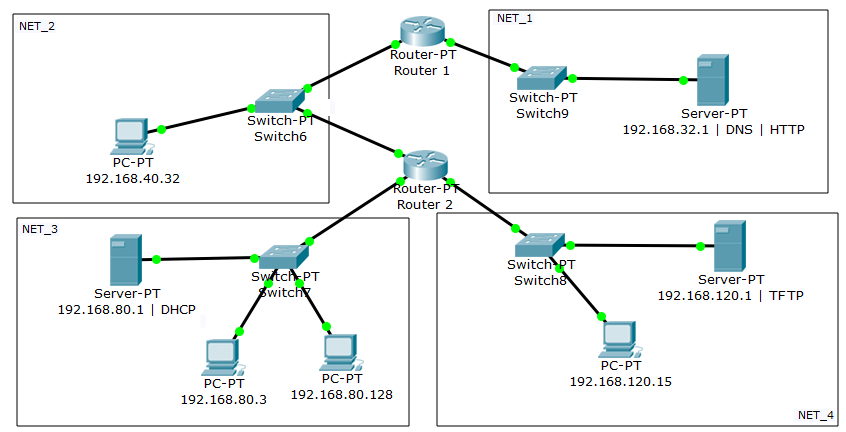
\includegraphics[width=\textwidth]{img/my_kks}
  \caption{Схема компьютерной сети}
\end{figure}
С помощью инструментов, были расставлены компьютеры, коммутаторы и роутеры типа \textbf{generic}, а также связаны между собой. По сравнению с работами в WMware, в данном случае:
\begin{itemize}
\item Вместо NetBSD и FreeBSD были использованы роутеры;
\item Вместо интернета выступает сервер с http страницой.
\end{itemize}


\tabulinesep = 1mm
\begin{longtabu} to \textwidth {|X[2, c , m ] |X[3,c , m ] | X[10, l, m ]|}\firsthline\hline
\textbf{Сегмент сети}&\textbf{Адрес узла}&\textbf{Описание}\\ \hline \endfirsthead
NET\_1&192.168.32.1&Сервер, с DNS и HTTP сервисами.\\ \hline
NET\_2&192.168.40.32&Компьютер, со статическим адресом.\\ \hline
NET\_3&192.168.80.1&Сервер, с DHCP сервисом.\\ \hline
NET\_3&192.168.80.3&Компьютер, адрес которого получен от DHCP сервера.\\ \hline
NET\_3&192.168.80.128&Компьютер, со статическим адресом.\\ \hline
NET\_4&192.168.120.1&Сервер, с TFTP сервисом.\\ \hline
NET\_4&192.168.120.15&Компьютер, со статическим адресом.\\ \hline
\caption{Описание узлов компьютерной сети}
\end{longtabu}

\subsection{Настройка адреса узла}
Для присвоения адреса какому-либо узлу, необходимо зайти в пункт \textbf{IP Configuration} и далее:
\begin{itemize}
\item Выбрать \textbf{DHCP}, если в сегменте сети имеется DHCP сервер;
\item Выбрать \textbf{Static}, если адрес предполагается статическим, и далее заполнить следующие поля:
\begin{itemize}
\item \textbf{IP Address};
\item \textbf{Subnet Mask};
\item \textbf{Default Gateway};
\item \textbf{DNS Server}.
\end{itemize}
\end{itemize}
После насктройки узла, для применения последних изменений рекомендуется перезагрузить его.

\subsection{Настройка сервисов}
Настройка DNS сервиса была произведена на узле с адресом 192.168.32.1. Для настройки необходимо выбрать, в меню настройки узла, пункт \textbf{DNS}, включить сервис и добавить новую запись. 

В данной работе была добавлена запись, со следующими параметрами:
\begin{itemize}
\item \textbf{name} - www.mypage.com
\item \textbf{address} - 192.168.32.1
\end{itemize}
То есть в данном случае, настраиваемый узел и является конечным узлом для данного доменного имени.

Также, для данного узла, был включен HTTP сервис, где уже имеется предварительно сгенерированная http-страница.\\\\
Настройка DHCP сервиса была произведена на узле с адресом 192.168.32.1. При которой были заполнены следующие поля:
\begin{itemize}
\item \textbf{Interface} - FastEthernet0;
\begin{itemize}
\item единственный интерфейс данного узла.
\end{itemize}
\item \textbf{Default Gateway} - 192.168.80.2;
\begin{itemize}
\item шлюзом по умолчанию выступает интерфейс роутера, подключенный к данной(NET\_3) подсети.
\end{itemize}
\item \textbf{DNS Server} - 192.168.32.1;
\begin{itemize}
\item предварительно настроенный DNS серверс из подсети NET\_1.
\end{itemize}
\item \textbf{Start IP Address} - 192.168.80.3;
\begin{itemize}
\item начала диапазона по выдаче IP-адресов.
\end{itemize}
\item \textbf{Subnet Mask} - 255.255.255.0;
\begin{itemize}
\item маска подсети.
\end{itemize}
\item \textbf{Maximun number of Users} - 100;
\begin{itemize}
\item максимальное количество пользователей.
\end{itemize}
\end{itemize}
Настройка TFTP сервиса была произведена на узле с адресом 192.168.120.15. Где его необходимо было включить, и для удобства удалить предварительно сгенерированные в нем файлы.


\subsection{Настройка роутеров}
В сети имеются два роутера(\textbf{Router 1} и \textbf{Router2}), которые выполняют функцию связующего звяна между подсетями.
\tabulinesep = 1mm
\begin{longtabu} to \textwidth {|X[c , m ] |X[c , m ] | X[c, m ]|}\firsthline\hline
\textbf{Роутер}&\textbf{Сеть}&\textbf{Адрес интерфейса}\\ \hline \endfirsthead
Router 1&NET\_1&192.168.32.128\\ \hline
Router 1&NET\_2&192.168.40.57\\ \hline
Router 2&NET\_2&192.168.40.2\\ \hline
Router 2&NET\_3&192.168.80.2\\ \hline
Router 2&NET\_2&192.168.120.2\\ \hline
\caption{Описание интерфейсов роутеров}
\end{longtabu}
Также, для корректной работы сети была добавлена маршрутизация. Для этого на Router 1, в настройках был выбран пункт \textbf{RIP Routing}, в который были добавлены следующие подсети:
\begin{itemize}
\item 192.168.32.0;
\item 192.168.40.0.
\end{itemize}
И для Router 2 соответственно:
\begin{itemize}
\item 192.168.40.0;
\item 192.168.80.0;
\item 192.168.120.0.
\end{itemize}

\section{Проверка}
\subsection{Проверка команды ping по адресу}
Откроем на узле 192.168.40.32(сеть NET\_2) утилиту \textbf{Command Prompt}, в которой введем команды \textbf{ipconfig} и \textbf{ping} в которой укажем адрес 192.168.120.15(сеть NET\_4).
\begin{lstlisting}[language={}]
C:\>ipconfig
FastEthernet0 Connection:(default port)
   Link-local IPv6 Address.........: FE80::2E0:A3FF:FEA3:7605
   IP Address......................: 192.168.40.32
   Subnet Mask.....................: 255.255.255.0
   Default Gateway.................: 192.168.40.2

C:\>ping 192.168.120.15
Pinging 192.168.120.15 with 32 bytes of data:
Reply from 192.168.120.15: bytes=32 time=1ms TTL=127
Reply from 192.168.120.15: bytes=32 time=1ms TTL=127
Reply from 192.168.120.15: bytes=32 time=1ms TTL=127
Reply from 192.168.120.15: bytes=32 time<1ms TTL=127

Ping statistics for 192.168.120.15:
    Packets: Sent = 4, Received = 4, Lost = 0 (0% loss),
Approximate round trip times in milli-seconds:
    Minimum = 0ms, Maximum = 1ms, Average = 0ms
\end{lstlisting}
Как видно из лога, команда пинг была успешна.

\subsection{Проверка команды ping по доменному имени}
Откроем на узле 192.168.80.3(сеть NET\_3) утилиту \textbf{Command Prompt}, в которой введем команды \textbf{ipconfig} и \textbf{ping} в которой укажем доменное имя \textbf{www.mypage.com}.
\begin{lstlisting}[language={}]
C:\>ipconfig
FastEthernet0 Connection:(default port)
   Link-local IPv6 Address.........: FE80::201:42FF:FE0B:D82B
   IP Address......................: 192.168.80.3
   Subnet Mask.....................: 255.255.255.0
   Default Gateway.................: 192.168.80.2

C:\>ping www.mypage.com
Pinging 192.168.32.1 with 32 bytes of data:
Reply from 192.168.32.1: bytes=32 time<1ms TTL=126
Reply from 192.168.32.1: bytes=32 time=10ms TTL=126
Reply from 192.168.32.1: bytes=32 time=11ms TTL=126
Reply from 192.168.32.1: bytes=32 time=13ms TTL=126

Ping statistics for 192.168.32.1:
    Packets: Sent = 4, Received = 4, Lost = 0 (0% loss),
Approximate round trip times in milli-seconds:
    Minimum = 0ms, Maximum = 13ms, Average = 8ms
\end{lstlisting}
Как видно из лога, доменное имя было преобразовано в адрес, по которому и была произведена команда ping.

\subsection{Проверка доступа к web странице}
На узле, с адресом 192.168.80.3(сеть NET\_3) была открыта утилита - браузер, в которой был введен адрес \textbf{www.mypage.com}.
\begin{figure}[H]
  \centering
  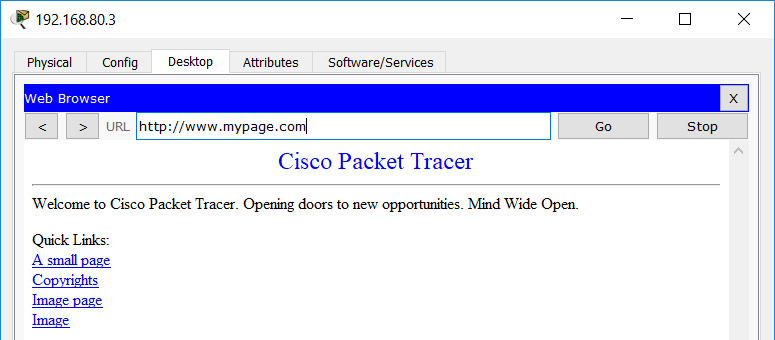
\includegraphics[width=.8\textwidth]{img/web}
  \caption{Web Browser}
\end{figure}
Как и ожидлось, страница была успешно загружена.

\subsection{Проверка TFTP}
На Router 2 была открыта консоль, в которой были выполнены следующие команды:
\begin{lstlisting}[language={}]
Router>enable
Router#show flash

System flash directory:
File  Length   Name/status
  3   5571584  pt1000-i-mz.122-28.bin
  2   28282    sigdef-category.xml
  1   227537   sigdef-default.xml
[5827403 bytes used, 58188981 available, 64016384 total]
63488K bytes of processor board System flash (Read/Write)

Router#copy flash tftp
Source filename []? pt1000-i-mz.122-28.bin
Address or name of remote host []? 192.168.120.1
Destination filename [pt1000-i-mz.122-28.bin]? temp.file

Writing pt1000-i-mz.122-28.bin...!!!!!!!!!!!!!!!!!!!!!!
[OK - 5571584 bytes]

5571584 bytes copied in 0.147 secs (8684467 bytes/sec)
\end{lstlisting}
Разберем действия:
\begin{enumerate}
\item Командой \textbf{enable} был совершен переход в привелегированный режим, можно заметить по символу решетки;
\item Командой \textbf{show flash} было выведено содержимое флеш-памяти, в данном случае это необходимо для тестовой загрузки по TFTP;
\item Командой \textbf{copy flash tftp} сообщаем о начале загрузке файла по tftp, где далее указывается файл(ы), tftp сервер для загрузки, а также новое имя файла(ов). 
\end{enumerate}
На TFTP сервере, в настройках TFTP появится выбранный ранее файл с указанным именем.



%На первичном сервере вводим команду \textbf{cat /etc/log/syslog}
%\begin{lstlisting}[language={}]
%...
%... zone example.com/IN: loaded serial 1
%... zone 40.168.192.in-addr.arpa/IN: loaded serial 1
%... zone 255.in-addr.arpa/IN: loaded serial 1
%... zone localhost/IN: loaded serial 2
%... all zones loaded
%... running
%... zone 40.168.192.in-addr.arpa/IN: sending notifies (serial 1)
%...
%\end{lstlisting}
%Как видно из части лога, зоны были успешно загружены и переданы на вторичный сервер.


\section*{Вывод}
В данной работе был получен опыт по работе в \textbf{Cisco Packet Tracer}.

По сравнению с прошлыми работами, где построение происходило с помощью WMware, в данном случае сеть была построена и настроена гораздо быстрее.

Построение и настройка были выполнены с помощью встроенных инструментов, которые в общем виде имитируют реальное оборудование. Если сравнивать с WMware, то в нем были рассмотрена настройка сети на конкретных системах(FreeBSD, NetBSD), в то время как в Cisco Packet Tracer это было сделано на лишь приближенных к реальности устройствах.

В общем случае Cisco Packet Tracer будет полезен при проектировании сети, но даст не так много опыта как WMware при настройке реальных систем.
%------------------------------------------------------------------------------

%\addcontentsline{toc}{section}{Список литературы}
%\bibliography{thesis}
%\bibliographystyle{ugost2008}

\end{document}